\documentclass[11pt,a4paper]{report}
\usepackage[textwidth=37em,vmargin=30mm]{geometry}
\usepackage{calc,xunicode,amsmath,amssymb,paralist,enumitem,tabu,booktabs,datetime2,xeCJK,xeCJKfntef,listings}
\usepackage{tocloft,fancyhdr,tcolorbox,xcolor,graphicx,eso-pic,xltxtra,xelatexemoji}

\newcommand{\envyear}[0]{2025}
\newcommand{\envdatestr}[0]{2025-03-14}
\newcommand{\envfinaldir}[0]{webdb/2025/20250314/final}

\usepackage[hidelinks]{hyperref}
\hypersetup{
    colorlinks=false,
    pdfpagemode=FullScreen,
    pdftitle={Web Digest - \envdatestr}
}

\setlength{\cftbeforechapskip}{10pt}
\renewcommand{\cftchapfont}{\rmfamily\bfseries\large\raggedright}
\setlength{\cftbeforesecskip}{2pt}
\renewcommand{\cftsecfont}{\sffamily\small\raggedright}

\setdefaultleftmargin{2em}{2em}{1em}{1em}{1em}{1em}

\usepackage{xeCJK,xeCJKfntef}
\xeCJKsetup{PunctStyle=plain,RubberPunctSkip=false,CJKglue=\strut\hskip 0pt plus 0.1em minus 0.05em,CJKecglue=\strut\hskip 0.22em plus 0.2em}
\XeTeXlinebreaklocale "zh"
\XeTeXlinebreakskip = 0pt


\setmainfont{Brygada 1918}
\setromanfont{Brygada 1918}
\setsansfont{IBM Plex Sans}
\setmonofont{JetBrains Mono NL}
\setCJKmainfont{Noto Serif CJK SC}
\setCJKromanfont{Noto Serif CJK SC}
\setCJKsansfont{Noto Sans CJK SC}
\setCJKmonofont{Noto Sans CJK SC}

\setlength{\parindent}{0pt}
\setlength{\parskip}{8pt}
\linespread{1.15}

\lstset{
	basicstyle=\ttfamily\footnotesize,
	numbersep=5pt,
	backgroundcolor=\color{black!5},
	showspaces=false,
	showstringspaces=false,
	showtabs=false,
	tabsize=2,
	captionpos=b,
	breaklines=true,
	breakatwhitespace=true,
	breakautoindent=true,
	linewidth=\textwidth
}






\newcommand{\coverpic}[2]{
    % argv: itemurl, authorname
    Cover photo by #2~~(\href{#1}{#1})
}
\newcommand{\makeheader}[0]{
    \begin{titlepage}
        % \newgeometry{hmargin=15mm,tmargin=21mm,bmargin=12mm}
        \begin{center}
            
            \rmfamily\scshape
            \fontspec{BaskervilleF}
            \fontspec{Old Standard}
            \fontsize{59pt}{70pt}\selectfont
            WEB\hfill DIGEST
            
            \vfill
            % \vskip 30pt
            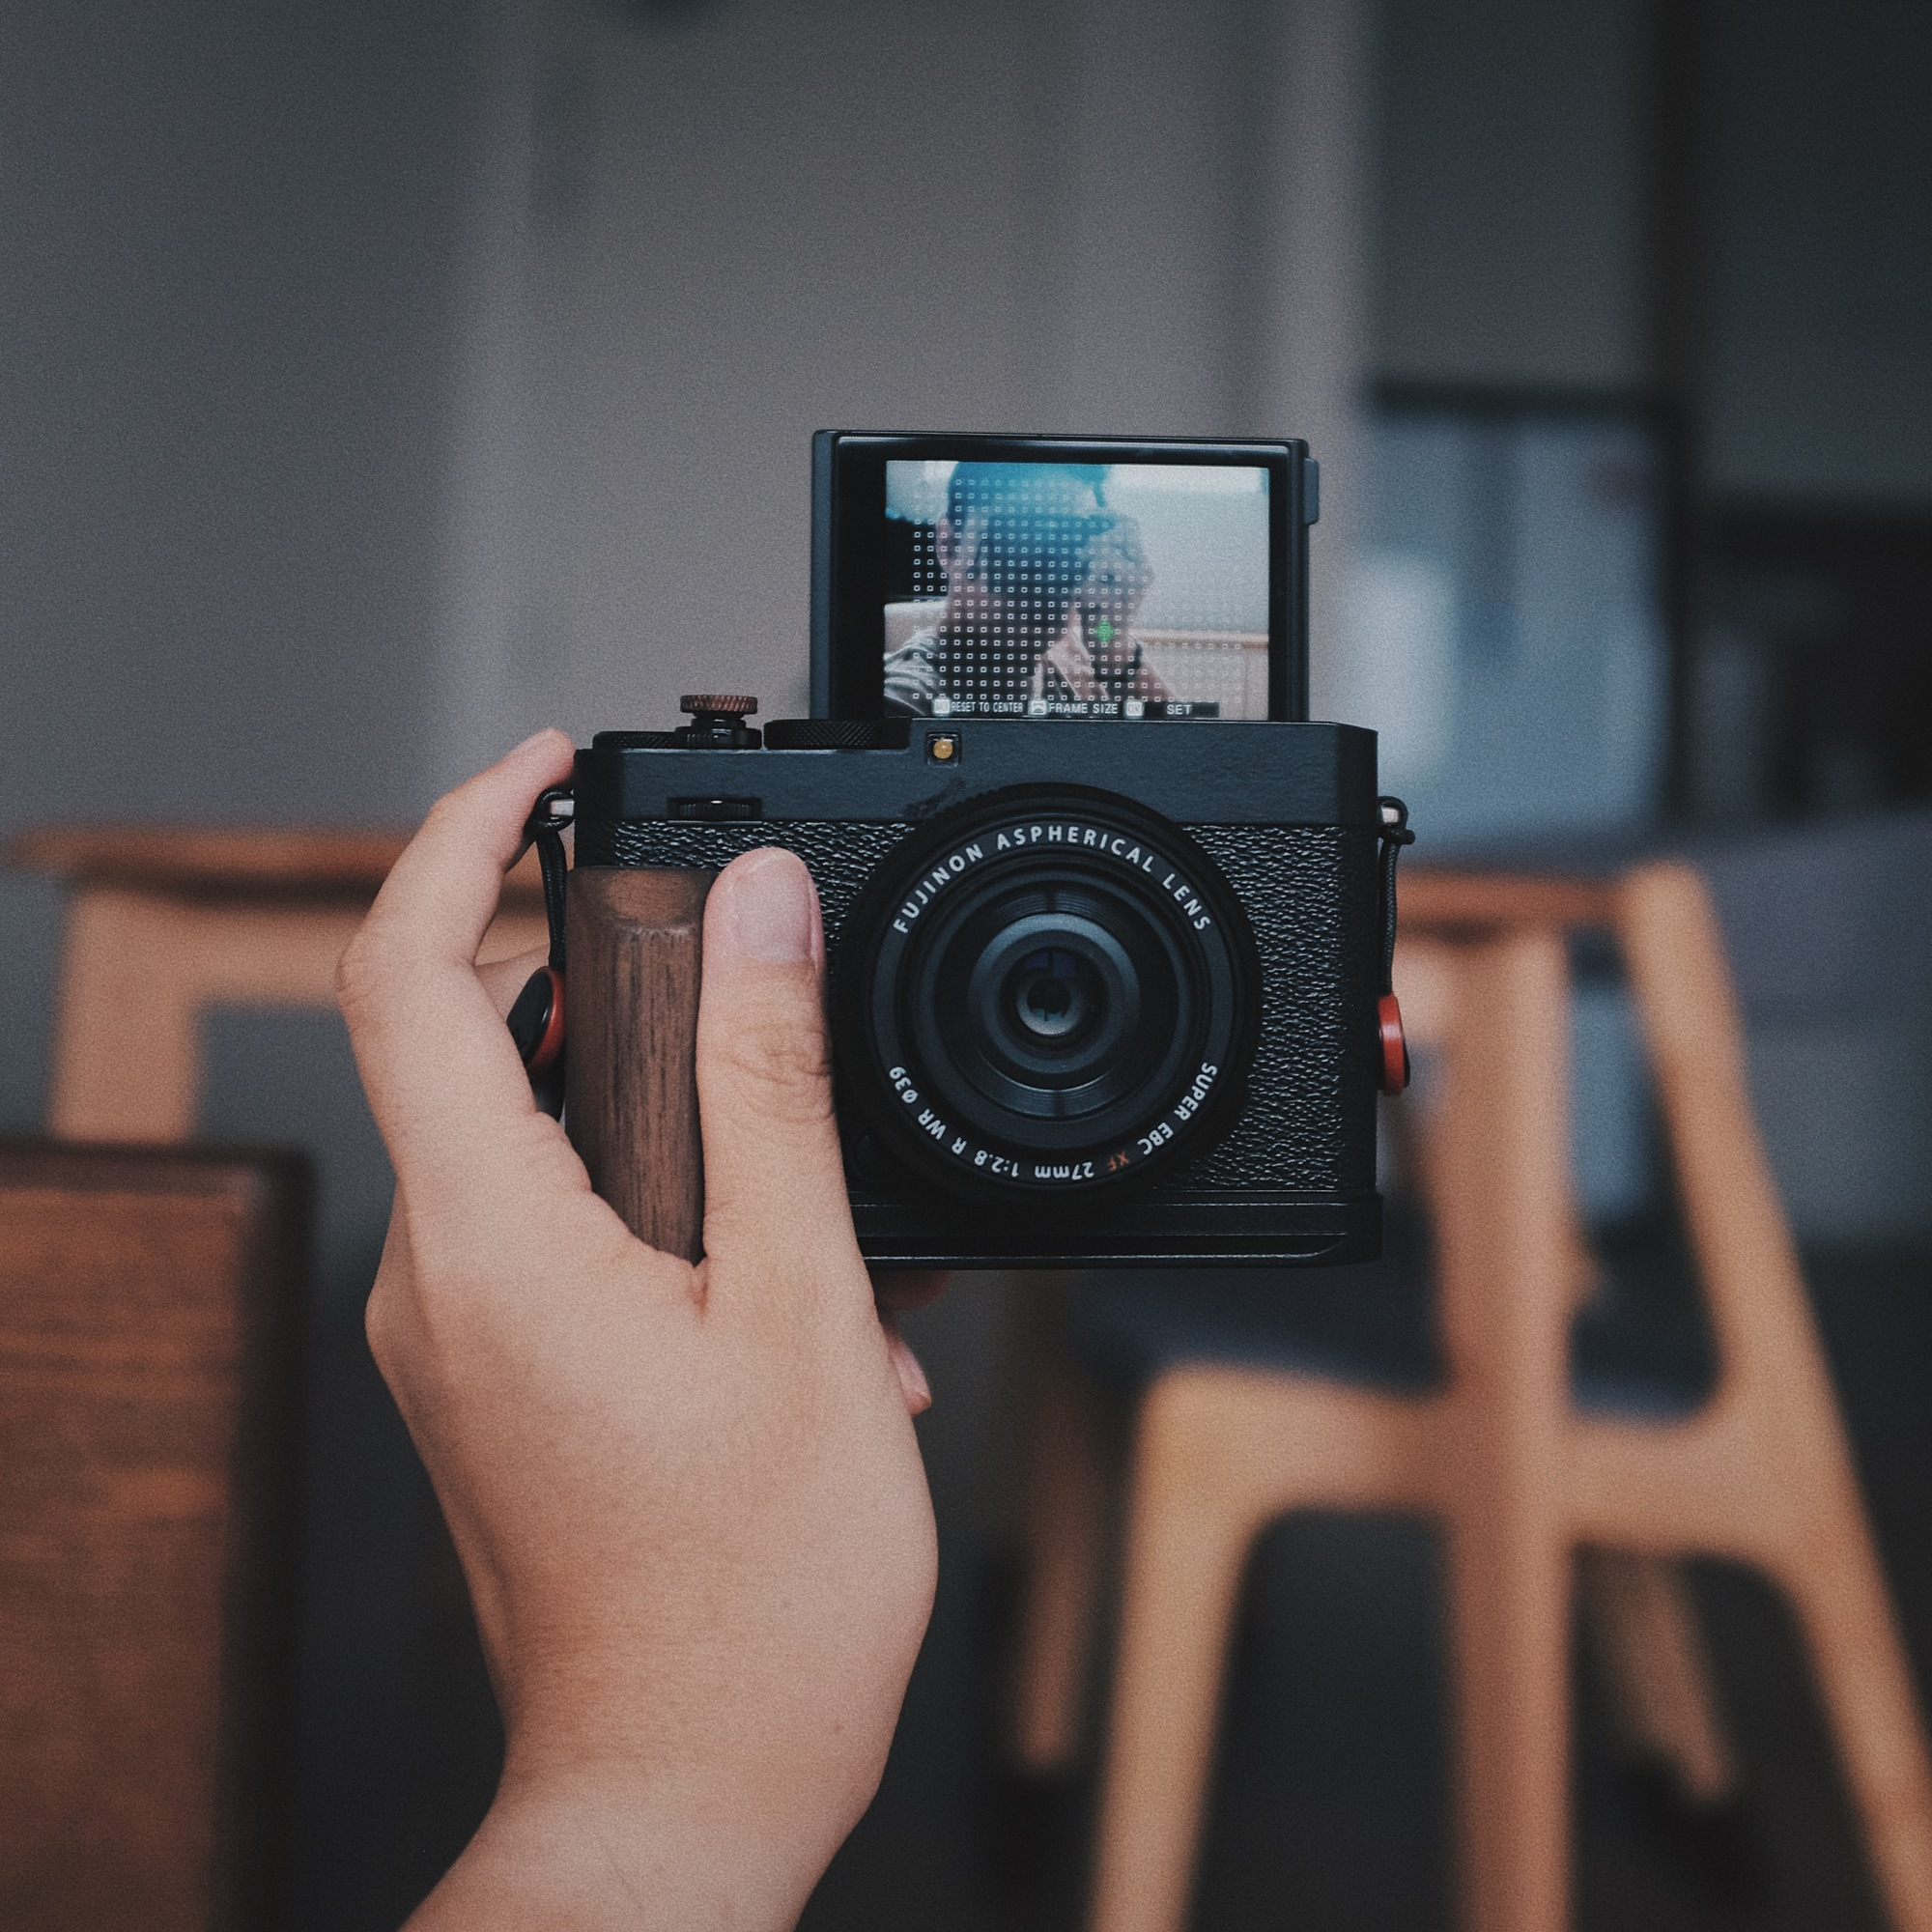
\includegraphics[width=\linewidth]{\envfinaldir/coverpic-prod.jpg}\par
            % \vskip 30pt
            \vfill

            \normalsize\rmfamily\scshape
            \copyright{} The Web Digest Project \hfill\large \envdatestr
        \end{center}
    \end{titlepage}
    % \restoregeometry
}
\newcommand{\simplehref}[1]{%
    \textcolor{blue!80!green}{\href{#1}{#1}}%
}
\renewcommand{\contentsname}{\center\Huge\sffamily\bfseries Contents\par\vskip 20pt}
\newcounter{ipartcounter}
\setcounter{ipartcounter}{0}
\newcommand{\ipart}[1]{
    % \vskip 20pt
    \clearpage
    \stepcounter{ipartcounter}
    \phantomsection
    \addcontentsline{toc}{chapter}{#1}
    % \begin{center}
    %     \Huge
    %     \sffamily\bfseries
    %     #1
    % \end{center}
    % \vskip 20pt plus 7pt
}
\newcounter{ichaptercounter}
\setcounter{ichaptercounter}{0}
\newcommand{\ichapter}[1]{
    % \vskip 20pt
    \clearpage
    \stepcounter{ichaptercounter}
    \phantomsection
    \addcontentsline{toc}{section}{\numberline{\arabic{ichaptercounter}}#1}
    \begin{center}
        \Huge
        \sffamily\bfseries
        #1
    \end{center}
    \vskip 20pt plus 7pt
}
\newcommand{\entrytitlefont}[1]{\subsection*{\raggedright\Large\sffamily\bfseries#1}}
\newcommand{\entryitemGeneric}[2]{
    % argv: title, url
    \parbox{\linewidth}{
        \entrytitlefont{#1}\par\vskip 5pt
        \footnotesize\ttfamily\mdseries
        \simplehref{#2}
    }\vskip 11pt plus 11pt minus 1pt
}
\newcommand{\entryitemGithub}[3]{
    % argv: title, url, desc
    \parbox{\linewidth}{
        \entrytitlefont{#1}\par\vskip 5pt
        \footnotesize\ttfamily\mdseries
        \simplehref{#2}\par\vskip 5pt
        \small\rmfamily\mdseries#3
    }\vskip 11pt plus 11pt minus 1pt
}
\newcommand{\entryitemAp}[3]{
    % argv: title, url, desc
    \parbox{\linewidth}{
        \entrytitlefont{#1}\par\vskip 5pt
        \footnotesize\ttfamily\mdseries
        \simplehref{#2}\par\vskip 5pt
        \small\rmfamily\mdseries#3
    }\vskip 11pt plus 11pt minus 1pt
}
\newcommand{\entryitemHackernews}[3]{
    % argv: title, hnurl, rawurl
    % \parbox{\linewidth}{
    %     \entrytitlefont{#1}\par\vskip 5pt
    %     \footnotesize\ttfamily\mdseries
    %     \simplehref{#3}\par
    %     \textcolor{black!50}{\href{#2}{#2}}
    % }\vskip 11pt plus 11pt minus 1pt
    \begin{minipage}{\linewidth}
            \entrytitlefont{#1}\par\vskip 5pt
            \footnotesize\ttfamily\mdseries
            \simplehref{#3}\par
            \textcolor{black!50}{\href{#2}{#2}}
    \end{minipage}\par\vskip 11pt plus 11pt minus 1pt
}







\begin{document}

\makeheader

\tableofcontents\clearpage




\ipart{Developers}
\ichapter{Hacker News}
\entryitemTwoLinks{"Normal" engineers are the key to great teams}{https://news.ycombinator.com/item?id=43356995}{https://spectrum.ieee.org/10x-engineer}

\entryitemTwoLinks{The Lost Art of Logarithms}{https://news.ycombinator.com/item?id=43356314}{https://www.lostartoflogarithms.com/}

\entryitemTwoLinks{Show HN: Bubbles, a vanilla JavaScript web game}{https://news.ycombinator.com/item?id=43355658}{https://ehmorris.com/bubbles/}

\entryitemTwoLinks{Honey Bunnies}{https://news.ycombinator.com/item?id=43355521}{https://mameson.com/experiment/glsl/fro\_9/fro\_9.html}

\entryitemTwoLinks{IO Devices and Latency}{https://news.ycombinator.com/item?id=43355031}{https://planetscale.com/blog/io-devices-and-latency}

\entryitemTwoLinks{Ask HN: Where do seasoned devs look for short-term work?}{https://news.ycombinator.com/item?id=43354115}{https://news.ycombinator.com/item?id=43354115}

\entryitemTwoLinks{Steam Networks}{https://news.ycombinator.com/item?id=43353822}{https://worksinprogress.co/issue/steam-networks/}

\entryitemTwoLinks{Statistical Formulas for Programmers (2013)}{https://news.ycombinator.com/item?id=43353551}{https://www.evanmiller.org/statistical-formulas-for-programmers.html}

\entryitemTwoLinks{Pirate Bay co-founder Carl Lundström has died}{https://news.ycombinator.com/item?id=43352580}{https://www.independent.co.uk/news/world/europe/pirate-bay-carl-lundstrom-dead-plane-crash-b2714284.html}

\entryitemTwoLinks{OpenAI asks White House for relief from state AI rules}{https://news.ycombinator.com/item?id=43352531}{https://finance.yahoo.com/news/openai-asks-white-house-relief-100000706.html}

\entryitemTwoLinks{Amateur Telescope Making Main Page}{https://news.ycombinator.com/item?id=43351988}{https://stellafane.org/tm/atm/}

\entryitemTwoLinks{Huawei targeted in new European Parliament corruption probe}{https://news.ycombinator.com/item?id=43351765}{https://www.ftm.eu/articles/huawei-targeted-in-european-parliament-corruption-probe}

\entryitemTwoLinks{Cursor told me I should learn coding instead of asking it to generate it}{https://news.ycombinator.com/item?id=43351137}{https://forum.cursor.com/t/cursor-told-me-i-should-learn-coding-instead-of-asking-it-to-generate-it-limit-of-800-locs/61132}

\entryitemTwoLinks{Doge Privacy Act Requests}{https://news.ycombinator.com/item?id=43349901}{https://jamieraskin.com/doge-privacy-act-requests/}

\entryitemTwoLinks{Meta is trying to stop a former employee from promoting her book about Facebook}{https://news.ycombinator.com/item?id=43349473}{https://www.engadget.com/social-media/meta-is-trying-to-stop-a-former-employee-from-promoting-her-book-about-facebook-004938899.html}

\entryitemTwoLinks{xlskubectl – a spreadsheet to control your Kubernetes cluster}{https://news.ycombinator.com/item?id=43349426}{https://github.com/learnk8s/xlskubectl}

\entryitemTwoLinks{My teen years: The transputer operating system}{https://news.ycombinator.com/item?id=43349214}{https://nanochess.org/transputer\_operating\_system.html}

\entryitemTwoLinks{'Uber for nurses' exposes 86K+ medical records, PII via open S3 bucket}{https://news.ycombinator.com/item?id=43349115}{https://www.websiteplanet.com/news/eshyft-report-breach/}

\entryitemTwoLinks{Something Is Rotten in the State of Cupertino}{https://news.ycombinator.com/item?id=43348891}{https://daringfireball.net/2025/03/something\_is\_rotten\_in\_the\_state\_of\_cupertino}

\entryitemTwoLinks{Practical UX for startups surviving without a designer}{https://news.ycombinator.com/item?id=43348379}{https://www.tibinotes.com/p/practical-ux-for-startups-surviving}\ichapter{Phoronix}
\entryitemGeneric{\hskip 0pt{}DXVK 2.6 Released With NVIDIA Reflex Support, Numerous Improvements}{https://www.phoronix.com/news/DXVK-2.6-Released}

\entryitemGeneric{\hskip 0pt{}Microsoft Releases March 2025 Update To Azure Linux 3.0}{https://www.phoronix.com/news/Azure-Linux-3.0.20250311}

\entryitemGeneric{\hskip 0pt{}Rusticl Wins: Mesa Officially Deprecates Clover OpenCL}{https://www.phoronix.com/news/Mesa-Deprecates-OpenCL-Clover}

\entryitemGeneric{\hskip 0pt{}NVIDIA RTX Remix 1.0 Released With DXVK DLSS4 \& Neural Radiance Cache}{https://www.phoronix.com/news/NVIDIA-RTX-Remix-1.0}

\entryitemGeneric{\hskip 0pt{}AMDVLK 2025.Q1.3 Brings Radeon RX 9070 Series Support}{https://www.phoronix.com/news/AMDVLK-2025.Q1.3-Released}

\entryitemGeneric{\hskip 0pt{}Intel Linux Graphics Driver Gets Patch To Help With Pixelflut Competition}{https://www.phoronix.com/news/Intel-Pixelflut-Patch-Linux-615}

\entryitemGeneric{\hskip 0pt{}Zed Editor Rolls Out Native Git Integration}{https://www.phoronix.com/news/Zed-Editor-Native-Git}

\entryitemGeneric{\hskip 0pt{}Mesa 25.1 To Enable Working Chromium VA-API Support}{https://www.phoronix.com/news/Mesa-Chromium-VA-API-MR}

\entryitemGeneric{\hskip 0pt{}Proposed Patches Would Allow Using Linux Kernel's libperf From Python}{https://www.phoronix.com/news/Linux-libperf-Python-RFC}\ichapter{Dribbble}
\entryitemGeneric{\hskip 0pt{}Tab Bar Animation}{https://dribbble.com/shots/25760227-Tab-Bar-Animation}

\entryitemGeneric{\hskip 0pt{}Carbon Solutions B2B Dashboard Design}{https://dribbble.com/shots/25681782-Carbon-Solutions-B2B-Dashboard-Design}

\entryitemGeneric{\hskip 0pt{}Logowave Awards Entry from Lepisov Branding}{https://dribbble.com/shots/25755190-Logowave-Awards-Entry-from-Lepisov-Branding}

\entryitemGeneric{\hskip 0pt{}Flare - Logo Design 🚀}{https://dribbble.com/shots/25754585-Flare-Logo-Design}

\entryitemGeneric{\hskip 0pt{}Bir-D / D.Bird}{https://dribbble.com/shots/25757221-Bir-D-D-Bird}

\entryitemGeneric{\hskip 0pt{}Squid Book}{https://dribbble.com/shots/25756273-Squid-Book}

\entryitemGeneric{\hskip 0pt{}Pricing Plan Web Page Design}{https://dribbble.com/shots/25755045-Pricing-Plan-Web-Page-Design}

\entryitemGeneric{\hskip 0pt{}Fishing Tournament Logo}{https://dribbble.com/shots/25750107-Fishing-Tournament-Logo}

\entryitemGeneric{\hskip 0pt{}Triceratops}{https://dribbble.com/shots/25749787-Triceratops}

\entryitemGeneric{\hskip 0pt{}Sergeant Scooper}{https://dribbble.com/shots/25749566-Sergeant-Scooper}

\entryitemGeneric{\hskip 0pt{}Atoms - Logo Concepts}{https://dribbble.com/shots/25749091-Atoms-Logo-Concepts}

\entryitemGeneric{\hskip 0pt{}Lamar® 21°}{https://dribbble.com/shots/25750164-Lamar-21}

\entryitemGeneric{\hskip 0pt{}Logo For Designed.supply}{https://dribbble.com/shots/25748434-Logo-For-Designed-supply}

\entryitemGeneric{\hskip 0pt{}Line Icons}{https://dribbble.com/shots/25749882-Line-Icons}

\entryitemGeneric{\hskip 0pt{}Codila Studio}{https://dribbble.com/shots/25749456-Codila-Studio}

\entryitemGeneric{\hskip 0pt{}Logo Database (V7) 2024—25}{https://dribbble.com/shots/25743610-Logo-Database-V7-2024-25}

\entryitemGeneric{\hskip 0pt{}Cullet LLC}{https://dribbble.com/shots/25750266-Cullet-LLC}

\entryitemGeneric{\hskip 0pt{}Crystal // Website}{https://dribbble.com/shots/25742820-Crystal-Website}

\entryitemGeneric{\hskip 0pt{}Sway}{https://dribbble.com/shots/25744097-Sway}

\entryitemGeneric{\hskip 0pt{}Emergency App Concept Design}{https://dribbble.com/shots/25711688-Emergency-App-Concept-Design}

\entryitemGeneric{\hskip 0pt{}Partify}{https://dribbble.com/shots/25040893-Partify}

\entryitemGeneric{\hskip 0pt{}OneC1 - Logo Design}{https://dribbble.com/shots/25732400-OneC1-Logo-Design}

\entryitemGeneric{\hskip 0pt{}Heyo® Monograms}{https://dribbble.com/shots/25732379-Heyo-Monograms}

\entryitemGeneric{\hskip 0pt{}Best Friends}{https://dribbble.com/shots/25730832-Best-Friends}


\ipart{Developers~~~~(zh-Hans)}
\ichapter{Solidot}
\entryitemGeneric{\hskip 0pt{}Google 称 Gemma 3 使用一张 H100 GPU 就能获得与 DeepSeek R1 相当的性能}{https://www.solidot.org/story?sid=80783}

\entryitemGeneric{\hskip 0pt{}D-Wave 称其量子退火处理器相比超算具有``量子优越性''}{https://www.solidot.org/story?sid=80782}

\entryitemGeneric{\hskip 0pt{}雄章鱼给雌性注射镇静剂以防止被吃掉}{https://www.solidot.org/story?sid=80781}

\entryitemGeneric{\hskip 0pt{}棕矮星的质量极限}{https://www.solidot.org/story?sid=80780}

\entryitemGeneric{\hskip 0pt{}沙特投资基金以 36 亿美元收购 Pokemon Go}{https://www.solidot.org/story?sid=80779}

\entryitemGeneric{\hskip 0pt{}英特尔任命陈立武为新 CEO }{https://www.solidot.org/story?sid=80778}

\entryitemGeneric{\hskip 0pt{}全球智能手表销量首次下滑}{https://www.solidot.org/story?sid=80777}

\entryitemGeneric{\hskip 0pt{}iRobot 警告它可能在 12 个月内倒闭}{https://www.solidot.org/story?sid=80776}

\entryitemGeneric{\hskip 0pt{}长时间玩游戏对幸福感影响不大}{https://www.solidot.org/story?sid=80775}

\entryitemGeneric{\hskip 0pt{}微软用 Windows App 替代 Remote Desktop app}{https://www.solidot.org/story?sid=80774}

\entryitemGeneric{\hskip 0pt{}至少 1.1 \% 的中世纪手稿是修女抄写的}{https://www.solidot.org/story?sid=80773}

\entryitemGeneric{\hskip 0pt{}Spotify 在 2024 年支付了 100 亿美元版税}{https://www.solidot.org/story?sid=80772}

\entryitemGeneric{\hskip 0pt{}Meta 开始测试其自研 AI 训练芯片}{https://www.solidot.org/story?sid=80771}

\entryitemGeneric{\hskip 0pt{}空气污染与生物衰老正相关,而绿地负相关}{https://www.solidot.org/story?sid=80770}

\entryitemGeneric{\hskip 0pt{}台积电提议与 AMD 等接管英特尔芯片制造业务}{https://www.solidot.org/story?sid=80769}

\entryitemGeneric{\hskip 0pt{}全球只有 7 个国家的 PM2.5 水平达到 WHO 的标准}{https://www.solidot.org/story?sid=80768}

\entryitemGeneric{\hskip 0pt{}TP-Link 高危漏洞被僵尸网络感染传播恶意程序}{https://www.solidot.org/story?sid=80767}

\entryitemGeneric{\hskip 0pt{}西班牙将对不标记 AI 生成内容的公司处以巨额罚款}{https://www.solidot.org/story?sid=80766}

\entryitemGeneric{\hskip 0pt{}Firefox 一根证书将于 2025 年 3 月 14 日过期}{https://www.solidot.org/story?sid=80765}

\entryitemGeneric{\hskip 0pt{}新西兰卫生部的财务管理系统是单张 Excel 表格}{https://www.solidot.org/story?sid=80764}\ichapter{V2EX}
\entryitemGeneric{\hskip 0pt{}[问与答] 净水器的挑选}{https://www.v2ex.com/t/1118303}

\entryitemGeneric{\hskip 0pt{}[计算机] 换电脑了,对于老电脑大家是怎么处理的?}{https://www.v2ex.com/t/1118302}

\entryitemGeneric{\hskip 0pt{}[宽带症候群] 90M 固定 IP 移动专线开通流水账记录}{https://www.v2ex.com/t/1118300}

\entryitemGeneric{\hskip 0pt{}[宽带症候群] 有开了移动到企的大佬吗?}{https://www.v2ex.com/t/1118299}

\entryitemGeneric{\hskip 0pt{}[Apple] 邮件 app 无法显示正文图片}{https://www.v2ex.com/t/1118298}

\entryitemGeneric{\hskip 0pt{}[DNS] 发现机场的审计规则可以用 DOH 绕过}{https://www.v2ex.com/t/1118297}

\entryitemGeneric{\hskip 0pt{}[远程工作] Flutter 跨平台开发工程师(招多名)}{https://www.v2ex.com/t/1118296}

\entryitemGeneric{\hskip 0pt{}[外汇交易] 求教,如何低汇率购买英镑?}{https://www.v2ex.com/t/1118295}

\entryitemGeneric{\hskip 0pt{}[Android] AndroidStudio Mac 无法启动 API19 的模拟器了吗?}{https://www.v2ex.com/t/1118293}

\entryitemGeneric{\hskip 0pt{}[程序员] my little story from 3\% to 100\%}{https://www.v2ex.com/t/1118292}

\entryitemGeneric{\hskip 0pt{}[买买买] 就是想入一个折叠}{https://www.v2ex.com/t/1118291}

\entryitemGeneric{\hskip 0pt{}[投资] v 站投资都比较理智,感觉做美股的比例要比雪球,股吧那边要多得多}{https://www.v2ex.com/t/1118290}

\entryitemGeneric{\hskip 0pt{}[分享创造] 在个人简介同步正在玩的 Steam 游戏}{https://www.v2ex.com/t/1118289}

\entryitemGeneric{\hskip 0pt{}[问与答] Cursor 刚注册的账号被风控了怎么办?}{https://www.v2ex.com/t/1118288}

\entryitemGeneric{\hskip 0pt{}[问与答] win11 有什么 免费 好用的手势识别软件吗?}{https://www.v2ex.com/t/1118287}

\entryitemGeneric{\hskip 0pt{}[问与答] 每日 LC 的今天题目几乎没有找到 AI 可以解出来}{https://www.v2ex.com/t/1118286}

\entryitemGeneric{\hskip 0pt{}[推广] 0.1 元领无限魔方小玩具 营销礼品}{https://www.v2ex.com/t/1118285}

\entryitemGeneric{\hskip 0pt{}[macOS] 大家有没有什么推荐的 可以在菜单栏出现时不遮挡字幕的 mac 本地播放器,比如字幕可以自动上移的.每次一按快进,菜单栏出现了,字幕全给挡了,菜单栏至少几秒才消失}{https://www.v2ex.com/t/1118283}

\entryitemGeneric{\hskip 0pt{}[分享创造] 自动答题(全新功能)| 自动签到 - 一亩三分地插件 耕地助手 更新了!}{https://www.v2ex.com/t/1118282}

\entryitemGeneric{\hskip 0pt{}[分享创造] [个人制作] 一个由大语言模型驱动的 AI 版德州扑克对战框架 - 来看大模型赛博斗蛐蛐~}{https://www.v2ex.com/t/1118281}

\entryitemGeneric{\hskip 0pt{}[Duolingo] 更新把我进度弄乱了}{https://www.v2ex.com/t/1118280}

\entryitemGeneric{\hskip 0pt{}[问与答] 在 2025 年 3 月的 iOS/iPadOS/macOS 中,如何用自然语言新建日历提醒事项?}{https://www.v2ex.com/t/1118279}

\entryitemGeneric{\hskip 0pt{}[问与答] 三星 s20, 使用微信发送语音消息声音变了, 如何恢复?}{https://www.v2ex.com/t/1118278}

\entryitemGeneric{\hskip 0pt{}[问与答] 老哥们一般怎么缓解愤怒情绪呢?}{https://www.v2ex.com/t/1118277}

\entryitemGeneric{\hskip 0pt{}[全球工单系统] firefox 下抖音直播每隔几分钟机会自动中断无限加载}{https://www.v2ex.com/t/1118275}

\entryitemGeneric{\hskip 0pt{}[MacBook] 一个没注意, Mac 电池最大容量只有 97\%了}{https://www.v2ex.com/t/1118274}

\entryitemGeneric{\hskip 0pt{}[职场话题] 中国广电咋样}{https://www.v2ex.com/t/1118273}

\entryitemGeneric{\hskip 0pt{}[生活] 过年相亲经历}{https://www.v2ex.com/t/1118272}

\entryitemGeneric{\hskip 0pt{}[职场话题] 从面试官的角度反思面试过程}{https://www.v2ex.com/t/1118271}

\entryitemGeneric{\hskip 0pt{}[问与答] steam 游戏下载的问题}{https://www.v2ex.com/t/1118270}

\entryitemGeneric{\hskip 0pt{}[问与答] 有没有会基于千川 API 来二次开发的}{https://www.v2ex.com/t/1118269}

\entryitemGeneric{\hskip 0pt{}[程序员] [找点逆向的思路] 找 GBA 版《星之卡比 梦之泉》的 当前关卡 内存地址}{https://www.v2ex.com/t/1118268}

\entryitemGeneric{\hskip 0pt{}[游戏主机] 首款 Xbox 品牌掌机的更多硬件规格泄露了}{https://www.v2ex.com/t/1118267}

\entryitemGeneric{\hskip 0pt{}[Kubernetes] 顺利成为 Kubestronaut 成员}{https://www.v2ex.com/t/1118265}

\entryitemGeneric{\hskip 0pt{}[分享发现] 请教下大家,现在还有没有活跃的游戏汉化、电影汉化的社区}{https://www.v2ex.com/t/1118264}

\entryitemGeneric{\hskip 0pt{}[程序员] 突然有点喜欢 Tauri 2.0 了}{https://www.v2ex.com/t/1118262}

\entryitemGeneric{\hskip 0pt{}[问与答] wise 现在不需要入金激活了?}{https://www.v2ex.com/t/1118261}

\entryitemGeneric{\hskip 0pt{}[宽带症候群] 山东联通宽带有办法提高上行带宽吗?}{https://www.v2ex.com/t/1118260}

\entryitemGeneric{\hskip 0pt{}[程序员] Ai 正在制造垃圾信息}{https://www.v2ex.com/t/1118258}

\entryitemGeneric{\hskip 0pt{}[Go 编程语言] Golang 实现的开源 NVR,中版 frigate,支持私有化部署}{https://www.v2ex.com/t/1118257}

\entryitemGeneric{\hskip 0pt{}[职场话题] 做什么能让自己快乐起来?}{https://www.v2ex.com/t/1118254}

\entryitemGeneric{\hskip 0pt{}[问与答] 有哪个性价比笔记高的公众号爬虫服务?}{https://www.v2ex.com/t/1118253}

\entryitemGeneric{\hskip 0pt{}[问与答] 最近装 KDE 进入桌面后所有面板都是空,添加控件界面也是空?}{https://www.v2ex.com/t/1118251}

\entryitemGeneric{\hskip 0pt{}[问与答] 求助, tensorflow lite 模型有什么 cli 工具可以打印它的基本信息吗}{https://www.v2ex.com/t/1118250}

\entryitemGeneric{\hskip 0pt{}[问与答] 求助,号码被别人用来刷单,频繁收到骚扰短信,格格爽存怎么屏蔽}{https://www.v2ex.com/t/1118249}

\entryitemGeneric{\hskip 0pt{}[Apple] [记录] iCloud Drive 随意删除我 5000+文件……以及找客服的后续}{https://www.v2ex.com/t/1118248}

\entryitemGeneric{\hskip 0pt{}[Python] 这是什么 jupyter 插件,感觉挺酷}{https://www.v2ex.com/t/1118246}

\entryitemGeneric{\hskip 0pt{}[分享发现] 主播是真赚钱呐, 70 万的关注,收入光打赏都 3 万多。}{https://www.v2ex.com/t/1118244}

\entryitemGeneric{\hskip 0pt{}[问与答] 大家有推荐开发人员入门快的原型设计工具吗?}{https://www.v2ex.com/t/1118242}

\entryitemGeneric{\hskip 0pt{}[问与答] 你们说话时鼻子不由自主的不通气吗?}{https://www.v2ex.com/t/1118239}


\ipart{Generic News}







\clearpage
\leavevmode\vfill
\footnotesize

Copyright \copyright{} 2023-2025 Neruthes and other contributors.

This document is published with CC BY-NC-ND 4.0 license.

The entries listed in this newsletter may be copyrighted by their respective creators.

This newsletter is generated by the Web Digest project.

The newsletters are also delivered via Telegram channel \CJKunderline{\href{https://t.me/webdigestchannel}{https://t.me/webdigestchannel}}.\\
RSS feed is available at \CJKunderline{\href{https://webdigest.pages.dev/rss.xml}{https://webdigest.pages.dev/rss.xml}}.

This newsletter is available in PDF at
\CJKunderline{\href{https://webdigest.pages.dev/}{https://webdigest.pages.dev/}}.

The source code being used to generate this newsletter is available at\\
\CJKunderline{\href{https://github.com/neruthes/webdigest}{https://github.com/neruthes/webdigest}}.

This newsletter is also available in
\CJKunderline{\href{http://webdigest.pages.dev/readhtml/\envyear/WebDigest-20250314.html}{HTML}} and
\CJKunderline{\href{https://github.com/neruthes/webdigest/blob/master/markdown/\envyear/WebDigest-20250314.md}{Markdown}}.


\coverpic{https://unsplash.com/photos/a-group-of-people-celebrating-with-colored-powder-and-confetti-OO\_AlBW8S3o}{Dibakar Roy}


\end{document}
